\section{Results}
%%%%%%%%%%%%%%%%%%%%%%%%%%%%%%%%%%%%%%%%%%%%%%%%%%%%%%%%%%%%%%%%%%%%%%
\label{sec:Results}

Once the signal strengths are extracted from the fit results, as explained in section \ref{sec:SignalExtraction}, and the uncertainties are decoupled the categories depicted in section \ref{sec:uncunf}, i.e. type A and type B uncertainties, we can go on unfolding the measured spectrum.
In figure \ref{fig:final_plot_preunf} is shown the $p_\mathrm{T, reco}^\mathrm{H}$ differential distribution before applying the unfolding procedure, compared with the MC truth expectation. The corresponding numbers are reported in table \ref{table:results_preunf}.

\begin{figure}[htb]
\centering
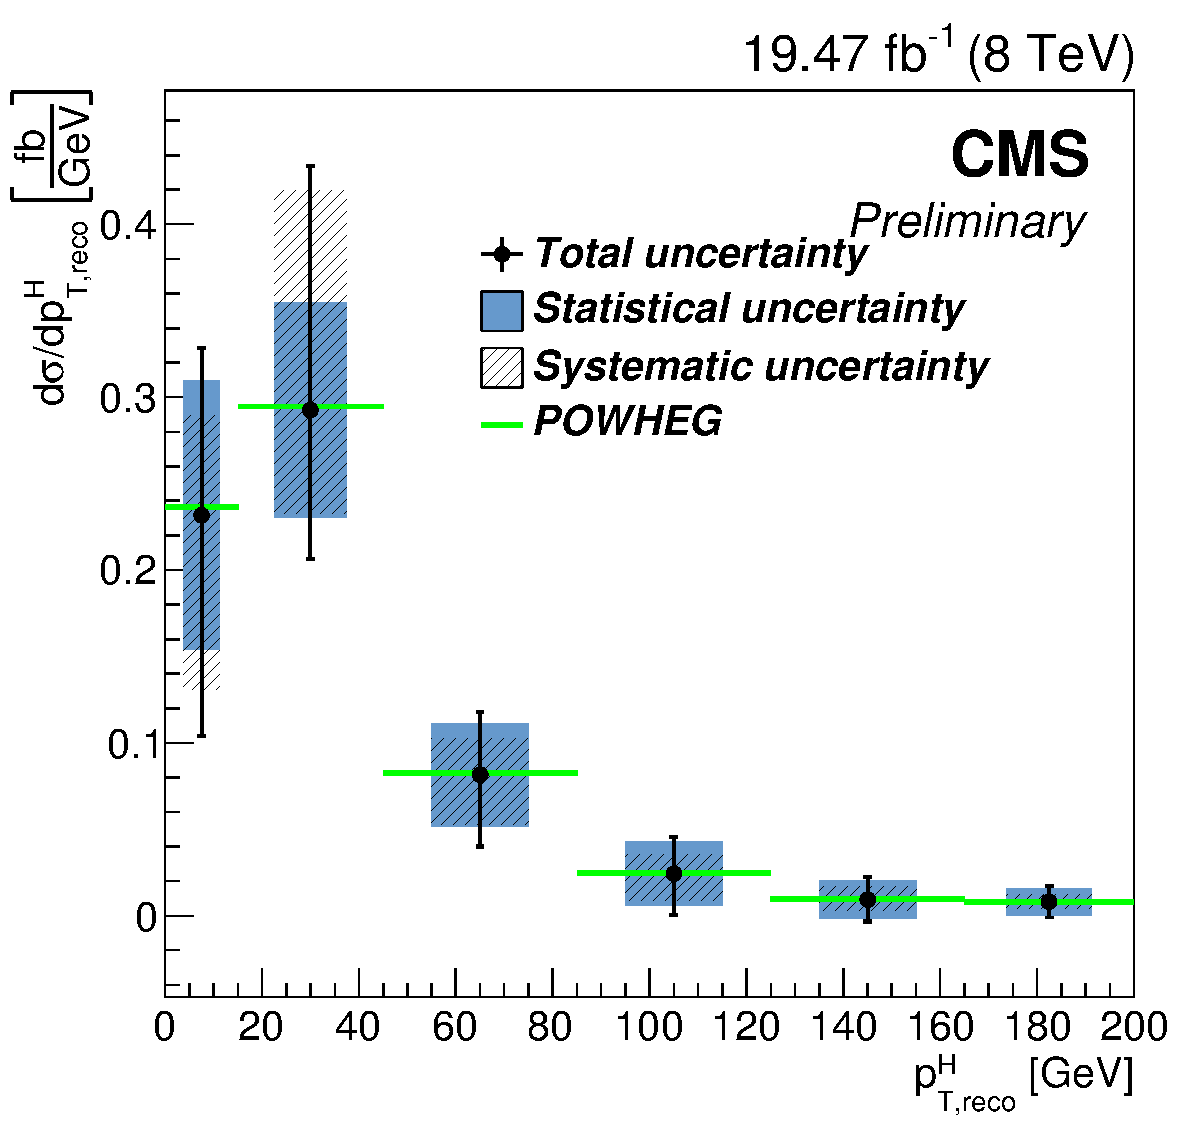
\includegraphics[width=0.7\textwidth]{images/plotsPreApp/preUnfolding.pdf}
\caption{Differential Higgs production cross section as a function of $p_\mathrm{T, reco}^\mathrm{H}$ before applying the unfolding procedure. The bins content corresponds to the MC prediction since the fit is performed on an Asimov dataset. The MC truth is represented by the green line.\label{fig:final_plot_preunf}}
\end{figure}

\begin{table}[htb]
\caption{Measured values for each bin of \pth with the corresponding total uncertainty compared with the MC truth expectation.}\label{table:results_preunf}
\centering
\begin{tabular}{c|ccccc}
Bin & Unfolded value & Total error(\%) & Stat error(\%) & Syst error(\%) & MC truth \\ 
\hline 
\hline 
1 & 0.23 & +41.9/-55.0 & $\pm$33.6 & +25.0/-43.5  &  0.24 \\ 
2 & 0.30 & +48.3/-29.5 & $\pm$21.3 & +43.3/-20.4  &  0.30 \\ 
3 & 0.08 & +44.8/-50.9 & $\pm$36.5 & +26.1/-35.4  &  0.08 \\ 
4 & 0.02 & +88.1/-99.1 & $\pm$75.9 & +44.8/-63.8  &  0.02 \\ 
5 & 0.01 & +141.1/-135.2 & $\pm$116.3 & +80.0/-68.9  &  0.01 \\ 
6 & 0.01 & +112.9/-110.6 & $\pm$99.5 & +53.3/-48.4  &  0.01 \\ 
\hline 
\end{tabular}
\end{table}

In order to unfold the spectrum, the procedure described in section \ref{sec:Unfolding} has been pursued.
The statistical plus type A systematic uncertainties are correctly propagated by the unfolding procedure into the final spectrum, taking into account the signal strenghts covariance matrix. The type B systematic uncertainty has been propagated using the following procedure: for each \pth bin, we compute the upper bound of the systematic band computing the square sum of all the signal strength variations that deviate in the up direction with respect to the bin central value, wether or not this variation correspond to the up or down shift of the nuisance. The same is done for the lower bound of the systematic band. If both the up and down shifts of a given nuisance leads to a same direction variation of the signal strength, only the larger variation is considered.\\
Results are reported in terms of a differential distribution, dividing by the luminosity (the uncertainty on the luminosity measurement is included in the statistical error band), and putting in each bin the bin content divided by the bin width.\\
In figure \ref{fig:final_plot} is shown the Higgs differential production cross section as a function of \pth. The results reported in this plot have been extracted fitting an Asimov dataset, thus the bins content corresponds to what expected from the MC predictions. The red shaded area in each bin represents the total uncertainty due to statistics plus systematics (type A and B). The blue area corresponds to the statistical error only. Data are not shown since the analysis is still blinded. As a cross check, the MC truth prediction has been superimposed to the plot. The final results are also shown in table \ref{table:results}. The systematic error reported in the table has been extracted in each been taking the difference of the squares of total and statistical error.\\
A comparison bewteen pre-unfolding and unfolded distributions shows that the relative uncertainties in each bin get reduced after the unfolding. To check the correctness of this result, a test using MC toys has been performed and is explained in Appendix \ref{app:toytest}.

\begin{figure}[htb]
\centering
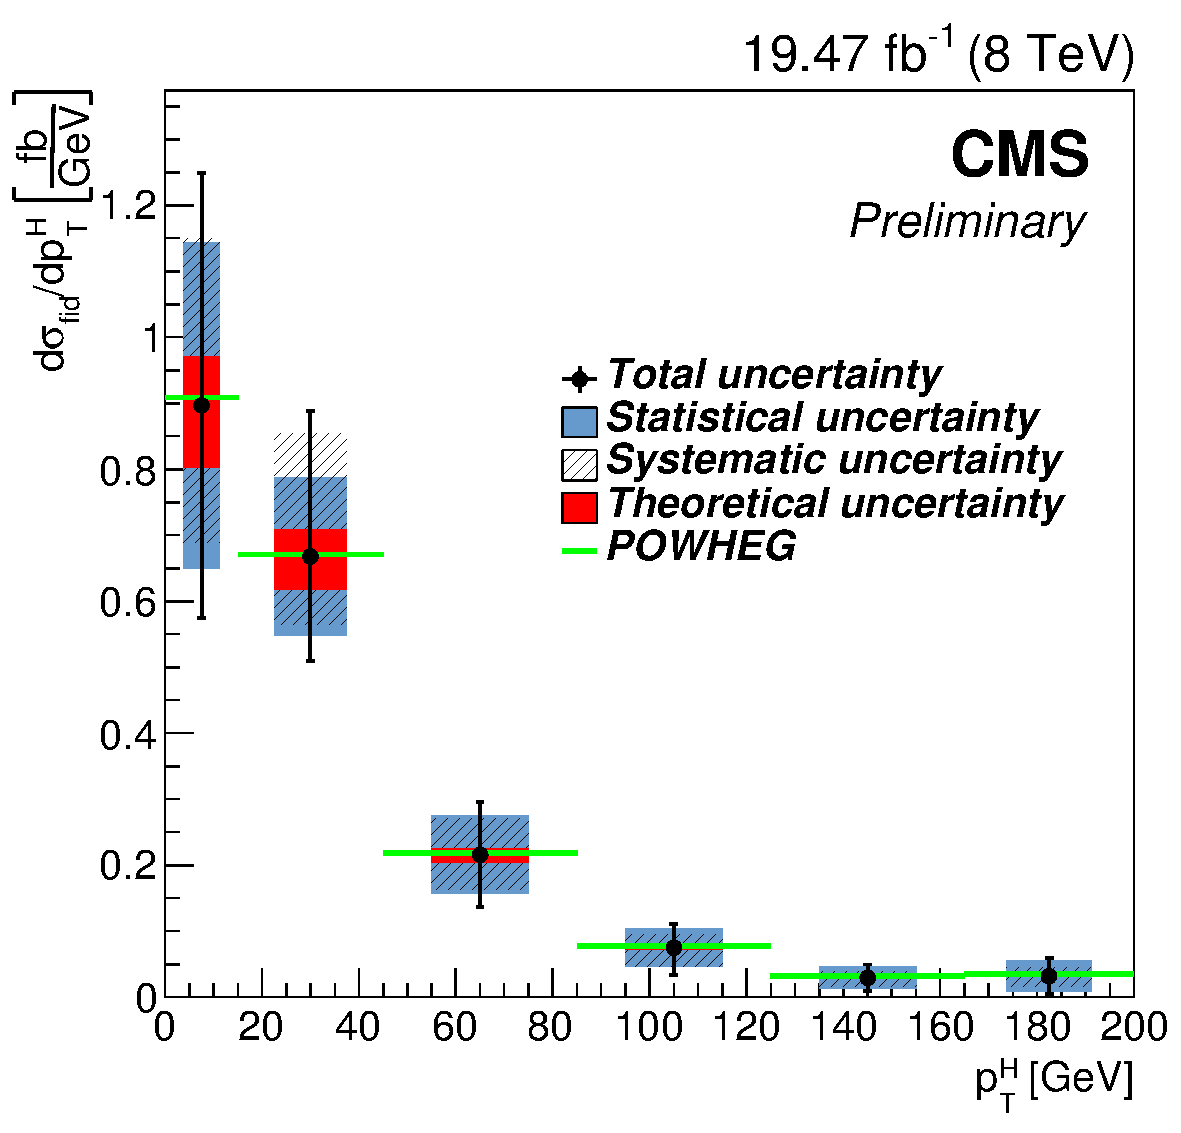
\includegraphics[width=0.7\textwidth]{images/plotsPreApp/unfolded_kreg3.pdf}
\caption{Unfolded differential Higgs production cross section as a function of \pth. The bins content corresponds to the MC prediction since the fit is performed on an Asimov dataset. The error bars are the total expected uncertainties in this measurement. Also the statistical, the systematic and the theoretical uncertainties are shown separately. The MC truth (POWHEG) is represented by the green histogram.\label{fig:final_plot}}
\end{figure}

\begin{table}[htb]
\caption{Unfolded values for each bin of \pth with the corresponding total uncertainty compared with the MC truth expectation.}\label{table:results}
\centering
\begin{tabular}{c|ccccc}
Bin & Unfolded value & Total error(\%) & Stat error(\%) & Syst error(\%) & MC truth \\ 
\hline 
\hline 
%1 & 0.90 & +37.7/-34.9 & $\pm$27.3 & +26.0/-21.7  &  0.91 \\ 
%2 & 0.67 & +31.7/-22.7 & $\pm$17.7 & +26.3/-14.2  &  0.67 \\ 
%3 & 0.22 & +36.2/-36.0 & $\pm$27.4 & +23.8/-23.4  &  0.22 \\ 
%4 & 0.07 & +47.7/-53.7 & $\pm$39.1 & +27.3/-36.8  &  0.08 \\ 
%5 & 0.03 & +66.0/-70.6 & $\pm$56.4 & +34.2/-42.5  &  0.03 \\ 
%6 & 0.03 & +86.2/-88.8 & $\pm$74.8 & +42.7/-47.8  &  0.03 \\ 
1 & 0.23 & +42.4/-55.4 & $\pm$ 34.0 & +25.3/-43.7  &  0.24 \\ 
2 & 0.29 & +48.7/-30.0 & $\pm$ 21.5 & +43.6/-20.9  &  0.29 \\ 
3 & 0.08 & +45.7/-51.9 & $\pm$ 36.9 & +26.9/-36.4  &  0.08 \\ 
4 & 0.02 & +88.5/-99.5 & $\pm$ 76.1 & +45.2/-64.1  &  0.02 \\ 
5 & 0.01 & +141.3/-135.3 & $\pm$ 116.4 & +80.1/-69.0  &  0.01 \\ 
6 & 0.01 & +112.9/-110.6 & $\pm$ 99.5 & +53.4/-48.4  &  0.01 \\ 
\hline 
\end{tabular}
\end{table}

Together with the unfolded spectrum, also the covariance matrix of the six bins is reported, in order to assess how much different bins are correlated. The result is shown in figure \ref{fig:cov_kreg3}.
\begin{figure}[htb]
\centering
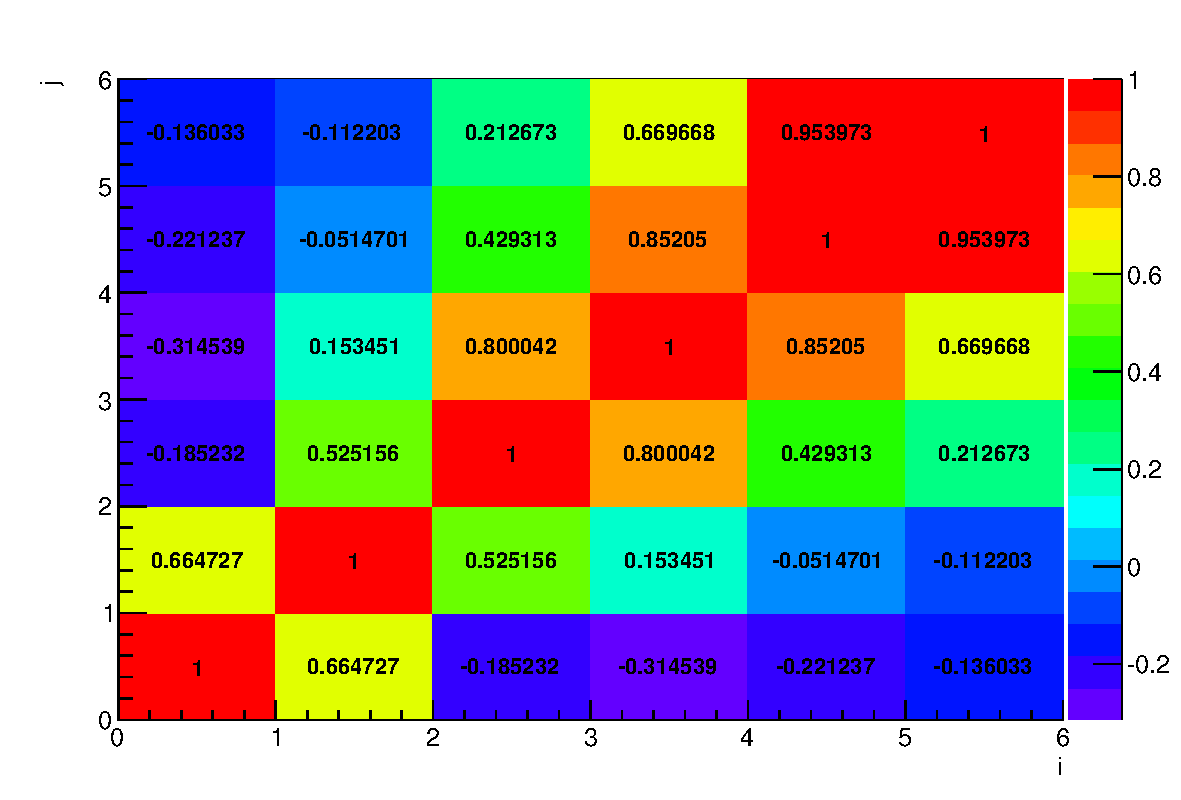
\includegraphics[width=0.7\textwidth]{images/plotsPreApp/covariance_kreg3.pdf}
\caption{Covariance matrix of the six \pth bins related to the unfolded distribution.\label{fig:cov_kreg3}}
\end{figure} 

The differential spectrum can be integrated to obtain a measurement of the inclusive cross section inside the fiducial region. The uncertainties can be correctly taken into account in this calculation using the covariance matrix of the six signal strengths to propagate the errors. In this case the unfolding procedure is not needed and to extrapolate the measured result to the fiducial region, only the efficiency of the analysis selection is needed.\\
%An alternative way is to repeat the fit procedure but considering one single signal strength, in this way all the nuisance parameters are correctly handled by the fit itself and we can extract asymmetric uncertainties. This latter procedure has been pursued to calculate the inclusive cross section.
 
The measured cross section after the analysis selection, i.e. number of events divided by luminosity, is $14 \pm 4~\mathrm{fb}$.
Using the overall efficiency defined in section \ref{subsec:EventSelection}, i.e. $\epsilon=0.362\pm{0.005}$, the cross section value in the fiducial region can be determined and is equal to:
\begin{equation}
%\sigma_{fid} = 47\pm 9~(stat)~^{+5}_{-5}~(syst)~\mathrm{fb} \quad . %%% Single mu method
\sigma_{fid} = 47\pm 7~(stat) \pm 9~(syst)~\mathrm{fb} \quad .
\end{equation}
As a closure test, the measurement can be extrapolated to the full $4\pi$ acceptance, using the efficiency reported in section \ref{subsec:EventSelection}, which is $\epsilon=0.03960\pm{0.00033}$.
The resulting cross section is:
\begin{equation}
%\sigma_{4\pi} = 496 \pm 97~(stat)~^{+56}_{-51}~(syst)~\mathrm{fb} \quad , %%% Single mu method
\sigma_{4\pi} = 433 \pm 67~(stat) \pm 83~(syst)~\mathrm{fb} \quad ,
\end{equation}
in agreement with the expected value from MC.
